%
% LaTeX report template 
%

% This is a comment: in LaTeX everything that in a line comes
% after a "%" symbol is treated as comment

\documentclass[11pt, a4paper]{article}
\usepackage{graphicx}
\usepackage{amsmath}
\usepackage{listings}
\usepackage{url}
\usepackage{float}
\usepackage{xcolor}

\definecolor{codegreen}{rgb}{0,0.6,0}
\definecolor{codegray}{rgb}{0.5,0.5,0.5}
\definecolor{codepurple}{rgb}{0.58,0,0.82}
\definecolor{backcolour}{rgb}{0.95,0.95,0.92}

\lstdefinestyle{mystyle}{
    backgroundcolor=\color{backcolour},   
    commentstyle=\color{codegreen},
    keywordstyle=\color{magenta},
    numberstyle=\tiny\color{codegray},
    stringstyle=\color{codepurple},
    basicstyle=\ttfamily\footnotesize,
    breakatwhitespace=false,         
    breaklines=true,                 
    captionpos=b,                    
    keepspaces=true,                 
    numbers=left,                    
    numbersep=5pt,                  
    showspaces=false,                
    showstringspaces=false,
    showtabs=false,                  
    tabsize=2
}

\lstset{style=mystyle}

\title{EE2703: Applied Programming Lab \\ Assignment No 7: Circuit Analysis using Sympy and Laplace Transforms} % Title

\author{Ishaan Agarwal \\ EE20B046} % Author name

\date{\today} % Date for the report
\begin{document}		
		
\maketitle % Insert the title, author and date

\section{Introduction}
The goal of this assignment is to understand the symbolic algebra capabilities of python and try and solve some circuits using the Laplace Transform. We also aim to understand the basics of the high pass and low pass filter circuits.

\section{Questions}
\subsection{Question 1}
To find the transfer function of the given circuit, and then find the unit step response:

\begin{figure}[H]
     \centering
     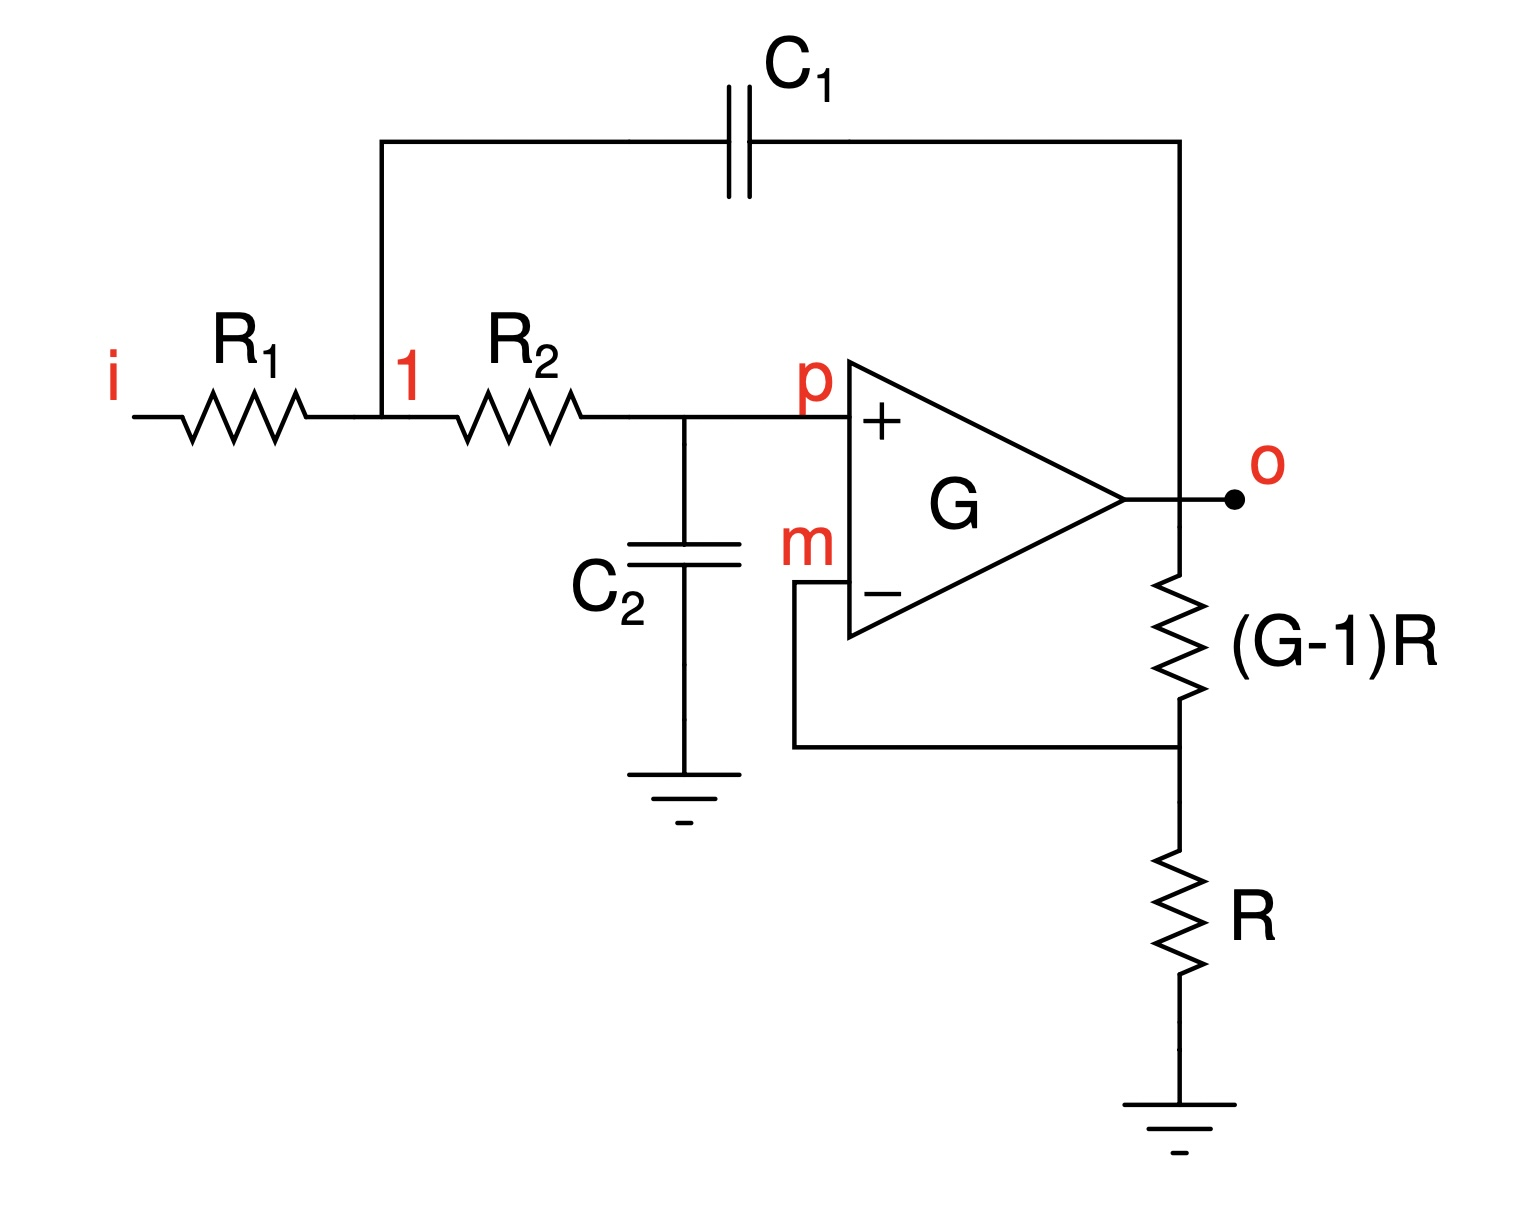
\includegraphics[scale=0.3]{Figure_0.png}
\end{figure}

Solving the circuit by using the basic KCL and KVL laws, we get the following solution in matrix form:

\[
\begin{bmatrix}
0 & 0 & 1 & -1/G\\
\frac{-1}{1+sc_2R_2} & 1 & 0 & 0\\
0 & -G & G & 1\\
-\frac{1}{R_1} -\frac{1}{R_2} - sC_1 & \frac{1}{R_2} & 0 & sC_1
\end{bmatrix}
\begin{bmatrix}
V1\\
Vp\\
Vm\\
V0
\end{bmatrix}
=
\begin{bmatrix}
0\\
0\\
0\\
-\frac{Vi(s)}{R_1}
\end{bmatrix}
\]

We then use the \texttt{sympy} library to implement this in python and also solve for the voltage vector.

We calculate the Voltage response for a unit input, which would thus give me the transfer function of this circuit. We then plot the Frequency response of this circuit. The following is the code:\\

\begin{lstlisting}[language = Python]
def lowpass(R1,R2,C1,C2,G,Vi):
    s=sp.symbols('s')
    #creating A and b matrices
    A = sp.Matrix([[0,0,1,-1/G],[-1/(1+s*R2*C2),1,0,0], [0,-G,G,1],[-1/R1-1/R2-s*C1,1/R2,0,s*C1]])
    b = sp.Matrix([0,0,0,-Vi/R1])
    #solving the system of equations using inverse
    V = A.inv() * b
    return (A, b, V)

A,b,V=lowpass(10000,10000,1e-9,1e-9,1.586,1) 
Vo=V[3] 
ww=np.logspace(0,8,801)
ss=1j*ww
s = sp.symbols('s')
hf=sp.lambdify(s,Vo,'numpy')
v=hf(ss)


plt.loglog(ww,abs(v))
plt.xlabel('Frequency')
plt.ylabel('Magnitude of H(jw)')
plt.title('Frequency Response of Low pass Filter')
plt.grid(True)
plt.show()
\end{lstlisting}
The following plot is obtained.

\begin{figure}[H]
     \centering
     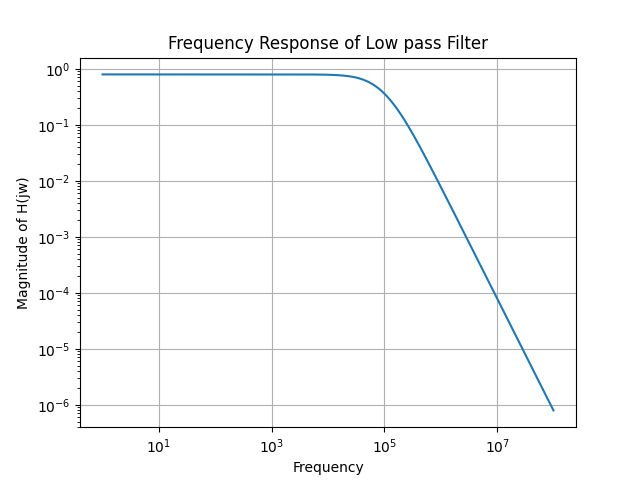
\includegraphics[scale=0.8]{Figure_1.png}
\end{figure}

Once we have obtained the system response in \texttt{sympy} symbolic form, we need to convert it to our standard \texttt{scipy.signal.lti} form in order to work with it further, the following function does this job.\\


\begin{lstlisting}[language = Python]
#defining a function to convert sympy transfer function polynomial to scipy lti system
def sympy_to_lti(xpr, s=sp.Symbol('s')):
    num, den = sp.simplify(xpr).as_numer_denom()  # expressions
    p_num_den = sp.poly(num, s), sp.poly(den, s)  # polynomials
    c_num_den = [sp.poly(p).all_coeffs() for p in p_num_den]  # coefficients
    l_num, l_den = [sp.lambdify((), c)() for c in c_num_den]  # convert to floats
    return sig.lti(l_num, l_den)
\end{lstlisting}

The unit step response of the circuit i.e the output for an input of $u(t)$ is calculated using the following code:\\

\begin{lstlisting}[language = Python]
#Question 1

#defining the lowpass filter 
A,b,V=lowpass(10000,10000,1e-9,1e-9,1.586,1/s) 
Vo=V[3]

Vo_s = sympy_to_lti(Vo)
t = np.linspace(0, 0.005, 100000)
t, y = sig.impulse(Vo_s, None, t)

#plot the unit step response
plt.plot(t, y)
plt.xlabel('Time (s)')
plt.ylabel('y(t)')
plt.title('Unit Step Response of Low pass Filter')
plt.grid(True)
plt.show()
\end{lstlisting}

The following plot is obtained:
\begin{figure}[H]
     \centering
     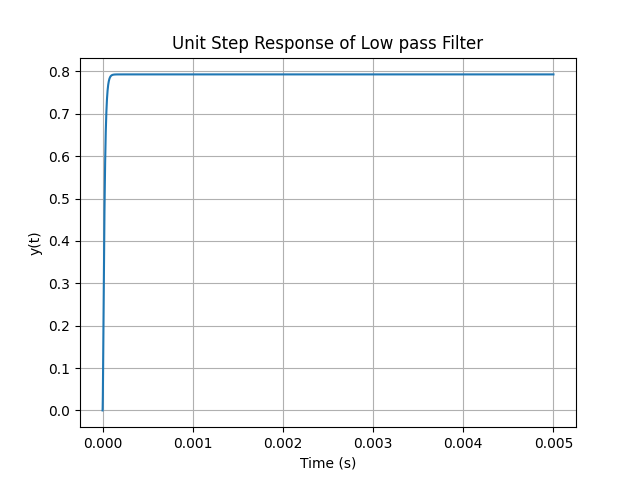
\includegraphics[scale=0.8]{Figure_2.png}
\end{figure}

\subsection{Question 2}
This time, we need to obtain the output for a mixed frequency input 
\[V_i(t) = (\sin(2000\pi t)+\cos(2*10^6\pi t))u_0(t) Volts\]

This is done as follows:\\
\begin{lstlisting}[language = Python]
#Question 2
#Obtaining the response for a mixed frequency input 

'''
Vi(t) = [sin(2000$\pi$t)+cos(2x10^6$\pi$t)]u0(t) Volts
'''

#low pass filter
a, b, V = lowpass(10000,10000,1e-9,1e-9,1.586,1)
Vo=V[3]
H = sympy_to_lti(Vo)
t = np.linspace(0, 0.005, 100000)
Vi = np.sin(2000*np.pi*t)+np.cos(2e6*np.pi*t)
t, y, svec = sig.lsim(H, Vi, t)

#plotting the input
plt.plot(t, Vi)
plt.plot(t, y, 'r')
plt.xlabel('Time (s)')
plt.ylabel('Vi(t)')
plt.title('Input and Output of Low Pass Filter')
plt.grid(True)
plt.legend(['Input','Output'])
plt.show()
\end{lstlisting}

The following plots are obtained:
\begin{figure}[H]
     \centering
     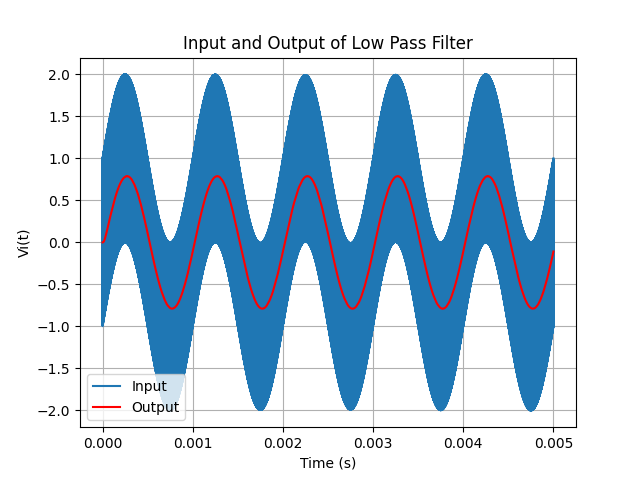
\includegraphics[scale=0.8]{Figure_5.png}
\end{figure}

This can be explained easily, since we know that a low pass filter only allows those frequencies to pass which are less than the pole frequency, i.e in this case $10^5$, thus the $10^3$ frequency component passes, whereas the $10^6$ frequency component is filtered out. \\Due to the very high frequency of the $10^6$ frequency signal, it appears as if this signal oscillates about the $10^3$ frequncy signal with the latter as it's mean value, in the input.

\subsection{Question 3}
Now, we try to do the same analysis for a high pass filter. A high-pass filter is a  filter that passes signals with a frequency higher than a certain cutoff frequency and attenuates signals with frequencies lower than the cutoff frequency. The circuit is as follows:

\begin{figure}[H]
     \centering
     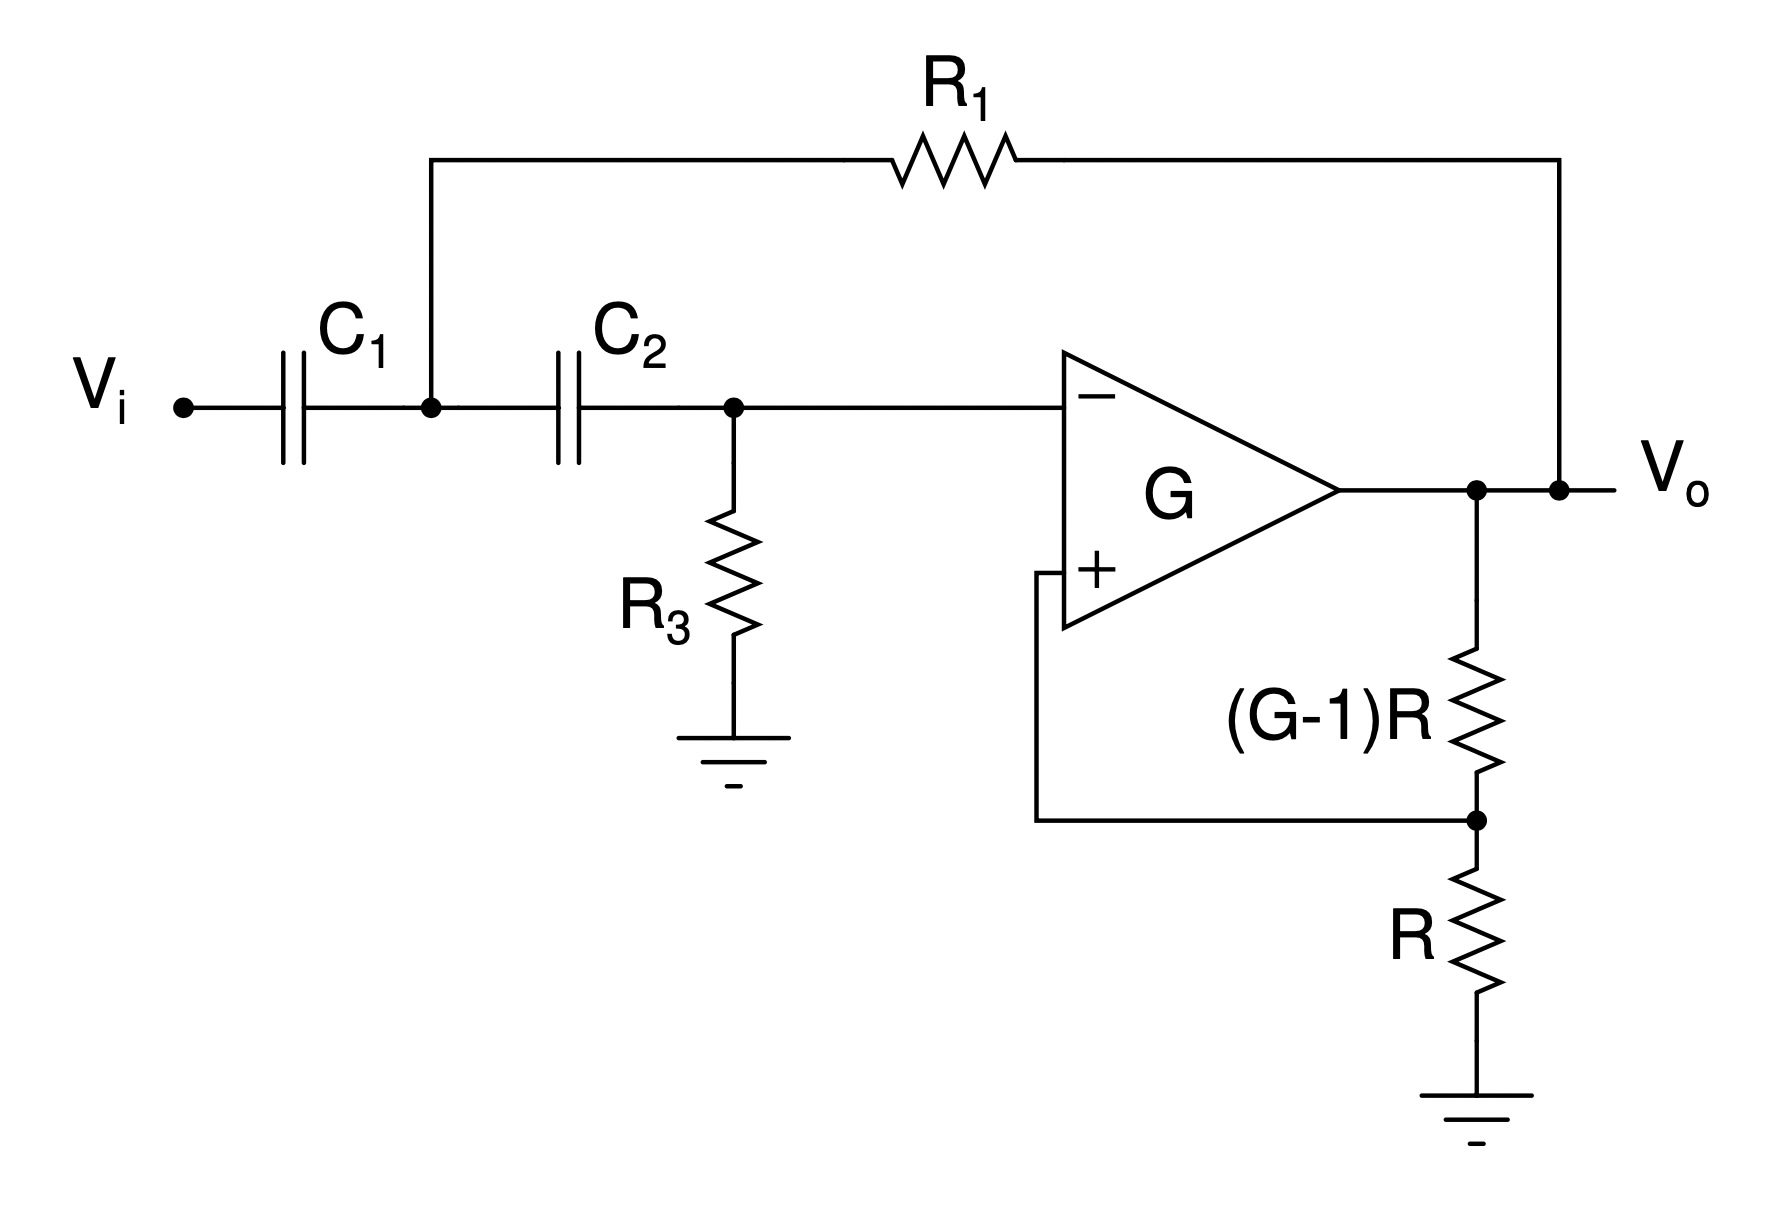
\includegraphics[scale=0.3]{Figure_8.png}
\end{figure}

The code for this part is as follows:\\
\begin{lstlisting}[language = Python]
#Question 3

def highpass(R1,R3,C1,C2,G,Vi):
    ''' High pass filter '''
    s=sp.symbols('s')
    A=sp.Matrix([[0,0,1,-1/G],[-1/(1+1/(s*R3*C2)),1,0,0],[0,-G,G,1],[-s*C1-s*C2-1/R1,s*C2,0,1/R1]])
    b=sp.Matrix([0,0,0,-Vi*s*C1])
    V = A.inv()*b
    return (A,b,V)

A,b,V=highpass(10000,10000,1e-9,1e-9,1.586,1) 
Vo=V[3] 
ww=np.logspace(0,8,801)
ss=1j*ww
s = sp.symbols('s')
hf=sp.lambdify(s,Vo,'numpy')
v=hf(ss)
plt.loglog(ww,abs(v))
plt.xlabel('Frequency')
plt.ylabel('Magnitude of H(jw)')
plt.title('Frequency Response of High Pass Filter')
plt.grid(True)
plt.show()


\end{lstlisting}

The following is the frequency response for the given high pass filter:

\begin{figure}[H]
     \centering
     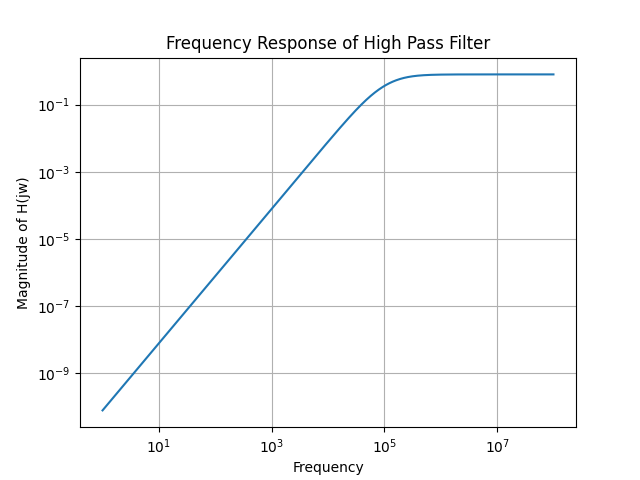
\includegraphics[scale=0.8]{Figure_3.png}
\end{figure}

\subsection{Question 4}
Now, we try to obtain the response of this filter for a damped sinusoidal input as follows:
\[V_{i1}(t) = e^{-5t} cos(2*\pi*10t)\] (f = 10)
\[V_{i2}(t) = e^{-50000t} cos(2*\pi*10^8*t) \] (f = $10^8$)

The code for this is as follows:\\
\begin{lstlisting}[language = Python]
#Question 4
#To obtain the response of the system for a damped sinusoid
'''
Vi1(t) = e^(-5t) cos(2*Pi*10t) (f = 10)
Vi2(t) = e^(-50000t) cos(2*Pi*10^8*t) (f = 10^8)
'''

A,b,V=highpass(10000,10000,1e-9,1e-9,1.586,1) 
Vo=V[3]
H = sympy_to_lti(Vo)

t1 = np.linspace(0, 1, 1000)
t2 = np.linspace(0, 0.0001, 1000)
vi1 = np.exp(-5*t1)*np.cos(2*np.pi*10*t1) #low frequency input
vi2 = np.exp(-50000*t2)*np.cos(2*np.pi*1e8*t2) #high frequency input

#finding the output of the high pass filter
t1, y1, svec = sig.lsim(H, vi1, t1)
t2, y2, svec = sig.lsim(H, vi2, t2)

#plotting the input and output for vi1
plt.plot(t1, vi1)
plt.plot(t1, y1, 'r')
plt.xlabel('Time (s)')
plt.ylabel('Input')
plt.title('Response of the High Pass Filter for low frequency input')
plt.grid()
plt.legend(['Input','Output'])
plt.show()

#plotting the input and output for vi2
plt.plot(t2, vi2)
plt.plot(t2, y2, 'r')
plt.xlabel('Time (s)')
plt.ylabel('Input')
plt.title('Response of the High Pass Filter for High frequency input')
plt.grid()
plt.legend(['Input','Output'])
plt.show()

\end{lstlisting}

The following graphs are obtained for the low frequency and high frequency inputs respectively.

\begin{figure}[H]
     \centering
     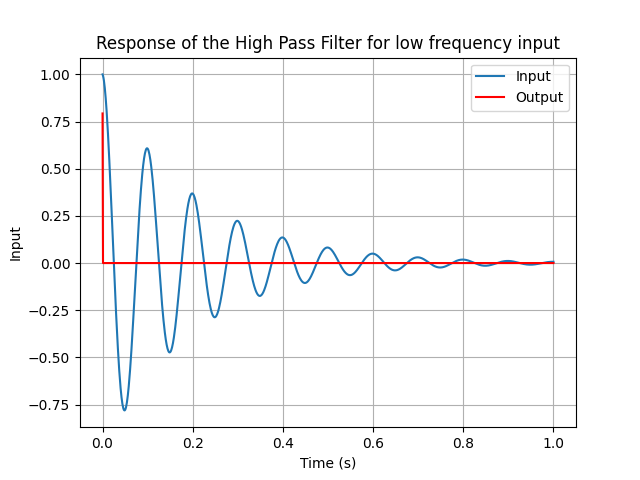
\includegraphics[scale=0.8]{Figure_6.png}
\end{figure}

\begin{figure}[H]
     \centering
     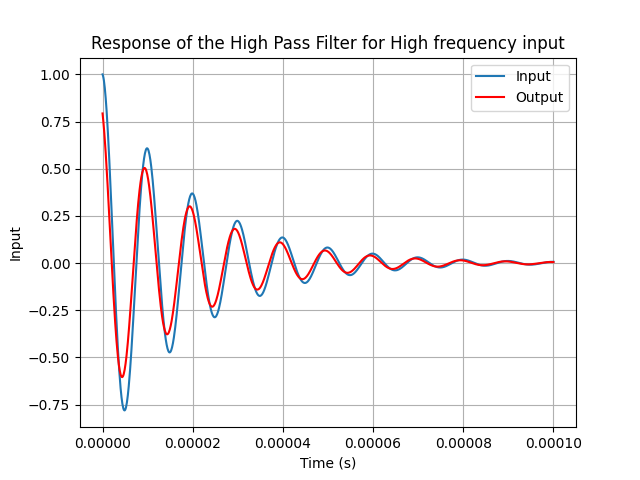
\includegraphics[scale=0.8]{Figure_7.png}
\end{figure}

This can be explained quite easily, we know that a high pass filter will not allow the frequency components lower than pole freuqency to pass. Thus, effectively the low frequency component is filtered and thus it is not observed in the output.\\
Whereas, in the high frequency input case, we see that the output is pretty much same as the input, which indicates that our filter is working as required.

\subsection{Question 5}
We aim to find the unit step response of the high pass filter. For this, we pass $u(t)$ (in Laplace domain 1/s) in the \texttt{highpass} function, and then compute the inverse Laplace using the \texttt{scipy.signal.impulse} function.
The following code does this:\\

\begin{lstlisting}[language = Python]
#Question 5

#defining the highpass filter 
A,b,V=highpass(10000,10000,1e-9,1e-9,1.586,1/s) 
Vo=V[3]

H = sympy_to_lti(Vo)
t = np.linspace(0, 0.001, 100000)
t, y = sig.impulse(H, None, t)

#plot the unit step response
plt.plot(t, y)
plt.xlabel('Time (s)')
plt.ylabel('y(t)')
plt.title('Unit Step Response of High Pass Filter')
plt.grid(True)
plt.show()

\end{lstlisting}

The following is the obtained response:
\begin{figure}[H]
     \centering
     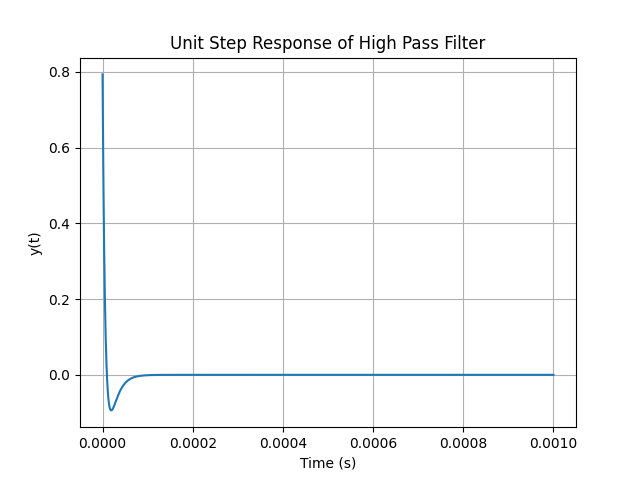
\includegraphics[scale=0.8]{Figure_4.png}
\end{figure}

Let's understand this response. As soon as the voltage is applied, i.e at t=$0^+$, the capacitors behave as short-circuited, and thus we see a positive voltage at the output node, whereas at t=$\infty$ (for practical purposes, this time is not that large), the capacitors would behave as open-circuited for DC-value of voltage and thus we would see zero volts at the output node.

\section{Conclusion}
In this assignment, we have understood the use of \texttt{sympy} library to do symbolic algebra. We have also learnt how this can be integrated with out previous knowledge of \texttt{scipy.signal} library to help solve circuits. We have also looked at some basic circuits like the high pass and the low pass filter and their responses for various inputs. 


\end{document}



 